\documentclass[prl,twocolumn,floatfix,superscriptaddress,nofootinbib,aps]{revtex4}
%\documentclass[11pt]{article}
\usepackage{amsfonts}
%\documentclass[usenatbib,11pt,a4paper,twoside]{article}
%\usepackage{epsfig,graphicx,times}
%\usepackage{amsmath}
%\usepackage{amssymb}
\usepackage{subfigure}
\usepackage{amssymb,amsmath,epsfig}
\usepackage{color}
\DeclareGraphicsExtensions{.eps,.png,.pdf,.jop}
%\DeclareGraphicsRule{.png}{eps}{.bb}{}

%\usepackage{geometry}
%\geometry{left=2.5cm,right=2.5cm,top=2.5cm,bottom=2.5cm}
%\setlength{\textwidth}{14.5true cm}

\def\hi{\textsc{Hi~}}

\def\mnras{Monthly Notices of the Royal Astronomical Society}
\def\apj{The Astrophysical Journal}
\def\apjl{Astrophysical Journal Letters}
\def\aap{Astronomy and Astrophysics}
\def\physrep{Physics Reports}
\def\jcap{Journal of Cosmology and Astroparticle Physics}
\def\prd{Physical Review D}
\def\pasj{Publications of the Astronomical Society of Japan}
\def\nat{Nature}
\def\apss{Astrophysics and Space Science}
\def\apjs{The Astrophysical Journal Supplement Series}
\def\aj{The Astronomical Journal}


\begin{document}

\title{Follow-up of one candidate 21 cm absorber found by blind searching}

%\author{{\large ......}}
%\date{}

%\begin{document}

%\today

\begin{abstract}
We request two sections of observing time at the 700 MHz -- 900 MHz band,
each with a 6 hours allocation, separated by four months, 
to follow up one 21 cm absorber candidate found in the 1hr GBT-field by our blind searching technique. 
This follow-up observation will allow us to demonstrate the blind searching technique for 21 cm absorbers. 
If confirmed, these would be the first HI absorbers detected through blind survey, instead of using 
an existing damped Lyman-alpha absorber (DLA) catalog. Observations of 21 cm absorption lines are expected 
to provide information on the gas properties of the absorber. We expect to constrain 
$N_{\rm HI}\,c_f/T_{\rm spin}$ (where $N_{\rm HI}$ is the column density of neutral hydrogen, 
$c_f$ is the covering factor, and $T_{\rm spin}$ is the spin temperature).
\end{abstract}

\maketitle
%\begin{document}
%\twocolumn

\section{The 21 cm absorption from cool neutral gas}
The 21 cm absorption traces the cool component of the neutral gas, 
which is the constituent material 
for star formation. The search for 21 cm absorption lines in damped 
Lyman-alpha absorbers (DLAs) has been successful 
\cite{2006MNRAS.370L..46K,2007MNRAS.375.1528K,2007MNRAS.382L..53Y,
2010MNRAS.402...35C,2014A&A...569A..35G,2011ApJ...727...52B,2015A&A...575A..44G}. 
These systems are believed to be the precursors of modern day galaxies, 
containing at least 80\% of the neutral gas mass density of the Universe
\cite{2005ApJ...635..123P}. The 21 cm absorption in DLAs can give a presentation of the physical conditions of the absorber, and these physical information of the absorbers at different redshifts can provide a new window for studying the galaxy evolution.  
Current 21 cm detections in DLAs have put constraints on $T_{\rm spin} /c_f$ 
(where $T_{\rm spin}$ is the spin temperature of neutral hydrogen, and 
$c_f$ is the covering factor), shedding light on the thermal status of 
the neutral gas. In particular, \citet{2010MNRAS.402...35C} provided evidence that the 
$T_{\rm spin}/c_f$ ratios seen at low redshift may also exist at high redshift, 
with a correlation between the 21 cm line strength and the total column density
of neutral hydrogen, $N_{\rm HI}$, indicating a roughly constant spin 
temperature/covering factor ratio for all of the DLAs searched.
\citet{2014A&A...569A..35G} constrains 
$N(\hi)c_f/T_{\rm spin}\sim(7.4\pm0.2)\times10^{18}\rm cm^{-2}$ with 
$27$ stacked absorption profiles at low redshift.

However, the number of the detected 21 cm absorbers is small, which limits the progression of the spin temperature detection.
And up to now, all the detections of 21 cm absorbers rely on the existing DLA 
catalogs. There may be a bias when we use the DLA catalog, which is not understood at present. Then a new searching technique apart from the DLA will be more reliable. As we show below, we have developed a blind searching technique 
to look for 21 cm absorbers directly from a 21 cm map, 
and found one candidate in the 1hr field GBT map. The confirmation 
enabled by a follow-up observation would demonstrate our blind searching 
technique, and provide the first 21 cm absorber detected by blind surveys. 
This technique could then be applied to future survey data, and search for 
more 21 cm absorbers. 

At the mean time, we can constrain the quantity $N_{\rm HI}\,c_f/T_{\rm spin}$
from the observed integrated optical depth, and see if there is any bias 
in the 21 cm absorbers detected in DLAs.


\section{The 21 cm absorber candidates from the 1hr field GBT map}
Our group has been actively engaged in a program of 21 cm intensity mapping by 
stacking and cross-correlation with field galaxies. The 1hr field data was 
collected as part of the AGBT10B\_036 allocation, and has been used
for cross-power spectrum and auto-power spectrum analysis 
\cite{2013MNRAS.434L..46S, 2013ApJ...763L..20M}.
Using the map made from the AGBT10B\_036 allocation, as well as the
AGBT13B\_352 and AGBT14B\_339,
we applied a blind searching technique and found 8 candidates absorber((1).RA = 0h54m00s, DEC = $1^{\circ}10^\prime$, 708.9661MHz, (2).RA = 0h36m41s, DEC = $3^{\circ}20^\prime$, 710.8948MHz, (3).RA = 1h02m39s, DEC = $3^{\circ}00^\prime$, 716.0217MHz (4).RA = 0h56m40s, DEC = $1^{\circ}40^\prime$, 744.4397MHz, (5).RA = 0h55m20s, DEC = $1^{\circ}10^\prime$, 751.9714MHz, (6).RA = 1h00m39s, DEC = $2^{\circ}10^\prime$, 767.9382MHz, (7).RA = 00h52m40s, DEC = $2^{\circ}00^\prime$, 771.2830MHz (8).RA = 1h05m20s, DEC = -$00^{\circ}10^\prime$, 777.8381MHz). Their spectra are showed in the appendix.

Because the data is collected through the whole year, the Doppler effect
of the Earth revolution around the Sun shifts the absorber frequency.
Considering such effect, the GBT data are separated into 5 time bins 
according to the magnitude of the influence of the Doppler effect, and converted to map domain respectively. Finally, different bins' maps are combined after Doppler effect corrected. We test the Doppler correction method with the known absorber in 3C286, and the results are shown in Fig. 1.

\begin{figure}[h!]
     \centering
     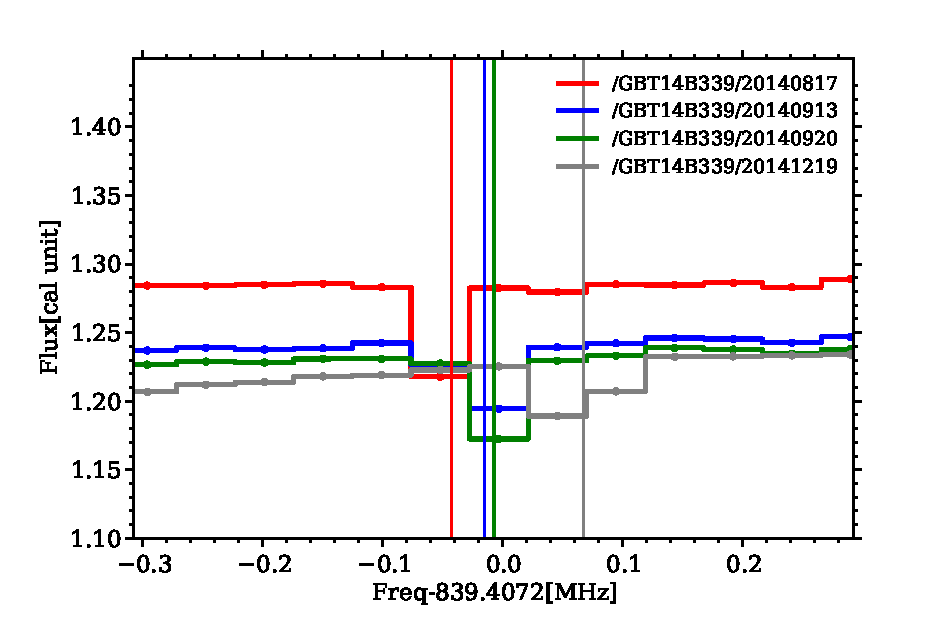
\includegraphics[width=9cm]{doppler_check01.eps}
     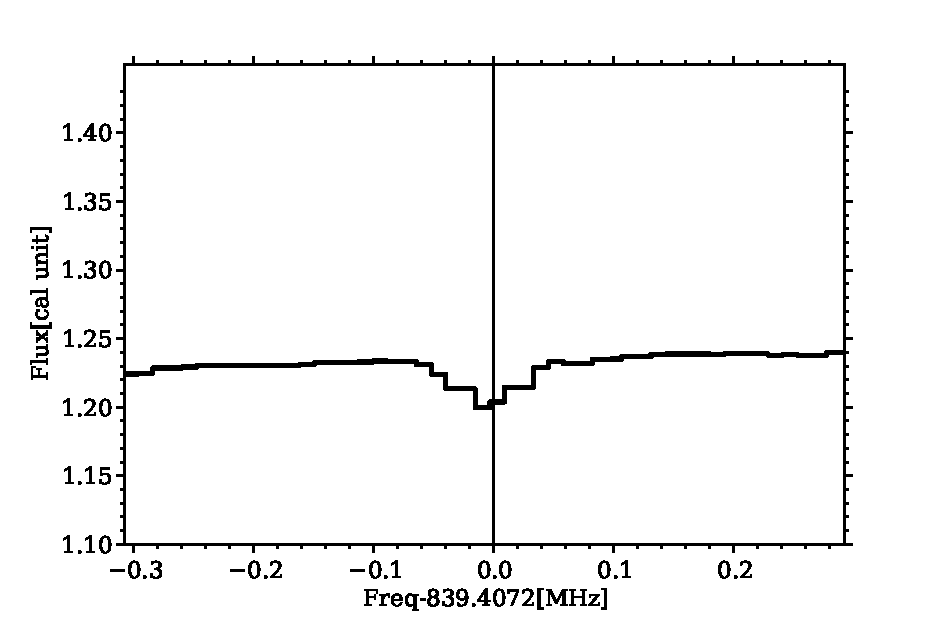
\includegraphics[width=9cm]{doppler_check02.eps}
     \caption{Test of the Doppler correction with known absorber in 3C286. Upper panel: the local spectrum of the known absorber observed in 4 days; the vertical lines indicate the Doppler shifted frequency of the absorber. Lower panel: the local spectrum of the absorber resulting from the combination of the 4 spectra after Doppler correction.}
     \label{doppler correction}
\end{figure}

The main steps of our absorber-finding technique are as follows. 
Firstly, we make the map of the observed sky with flag and svd algorithm, which can remove most of the noise. Secondly, for each of the pixel's spectrum data, we use two ways to fitting the spectrum and obtained the mean value and the absorption signal. One of it is using an intermediate frequency filter to fit the spectrum, in the other way, for each point in the spectrum we combine it with its neighbor points and use least square method to compute the mean value and the absorption signal. For the data resulted from the two fitting ways, we process both of them by the following procedure. Then, we compute the noise of each pixels' data in all frequency and use it as the standard deviation, and select all the frequency bins with absorption signal higher than $3\, \sigma$, for each spatial pixel. Finally, we check all the trough we select in the spectrum, and choose the one that has a reasonalble absorptional line profile with its neighbouring points as the absorber candidates.

However, there are too many candidates left and we carry out the following check to find the ideal candidates. As a first check, if there are too many candidates in one frequency bin distributed at various pixels, or the distribution of them is regular, we eliminate these candidates. Then as a second check, we divide the original data into two sections in the integration time, both of which have the same frequency range and spatial field and nealy half the integration time as the original data. We do the blind searching process described above again on each of the section map. Only the candidates that show up on both sections are survived. Finally as a third check, to exclude the uncertainty induced by the way how we devide the oringinal data, we do the second check again with a different deviding way. Only the candidates that survives all the check are selected as the real candidates.

After all the check, we select the exact candidates that can be found from searching with different fitting ways.

Finally, for the confidence level we choose the candidates have S/N lager than 5.0 and have consistent absorption flux in spectra from all five doppler bins. Then there is eight left. The local spectra of this candidate after subtracting the continuum is shown in the appendix.
If the candidates are confirmed, we would like to apply our blind searching method
to other fields of our data sets.


%\begin{figure*}[htpb]
%\centering{
%\subfigure[]{
%    \includegraphics[width=6cm]{png/abs771.png}
%}
%\subfigure[]{
%    \includegraphics[width=6cm]{png/abs867.png}
%}
%\subfigure[]{
%     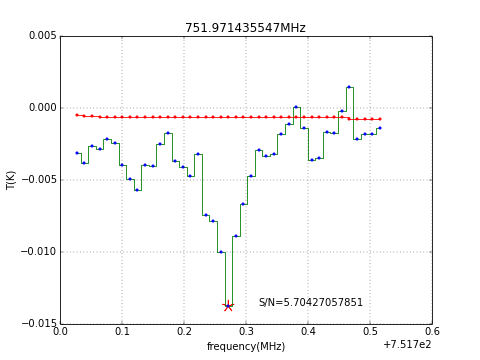
\includegraphics[width=6cm]{751971435_22_7_svd.png}
%}
%\caption{
%    (Absorber found last time)
%    The local spectra of two 21 cm absorber candidates after 
%    subtracting the continuum. {\it Left panel:} 
%    The candidate absorber at 771.240 MHz. {\it Right panel:} 
%    The candidate absorber at 867.773 MHz.}
%    }
%\label{Fig.candidates}
%}
%\end{figure*}

%\begin{figure}[h!]
%      \centering
%      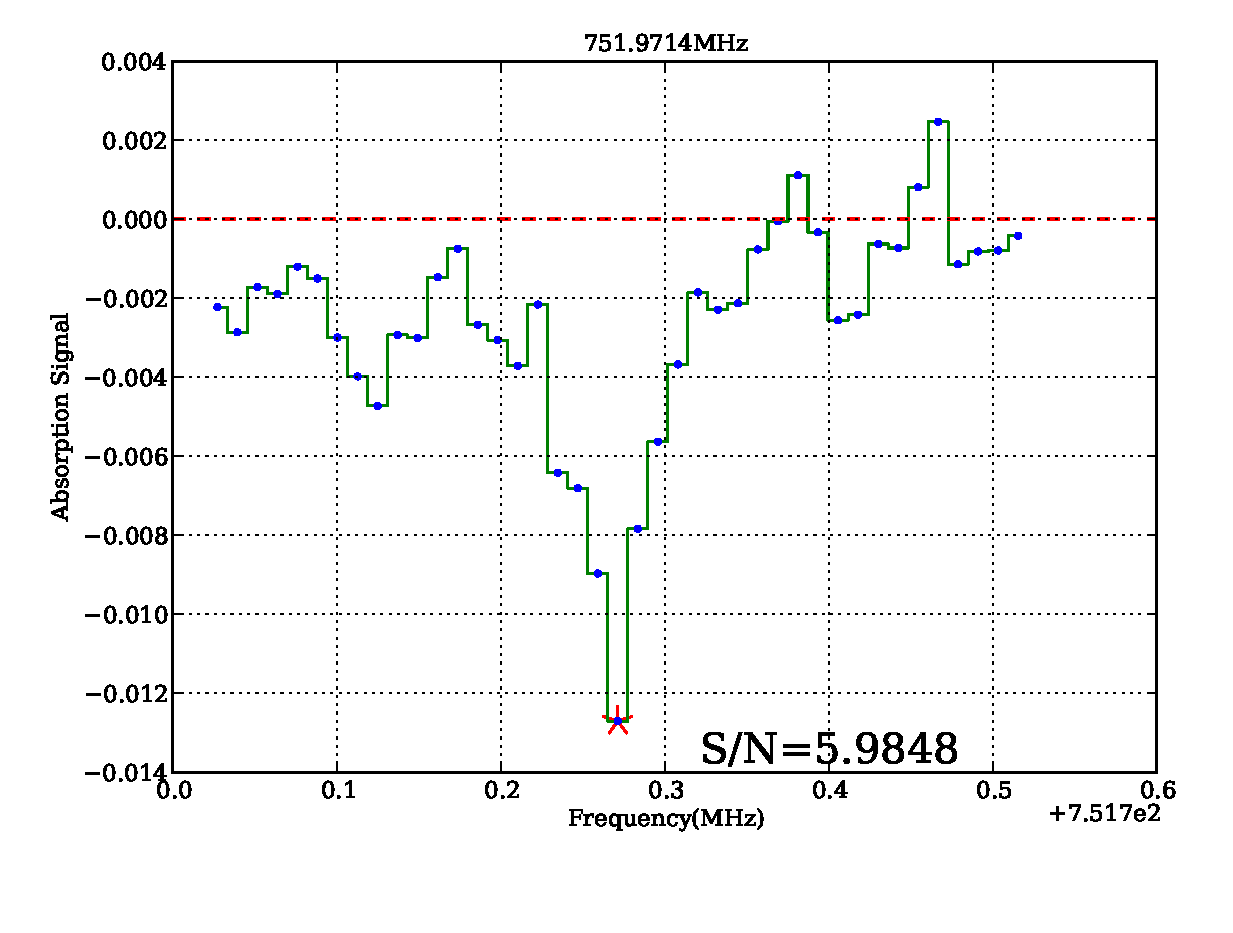
\includegraphics[width=8cm]{751971435_22_7_svd.eps}
%      %\caption{The local spectra of two 21 cm absorber candidates after subtracting the continuum.}
%      %\label{Fig.candidates}
%\end{figure}
%\begin{figure}[h!]
%      \centering
%      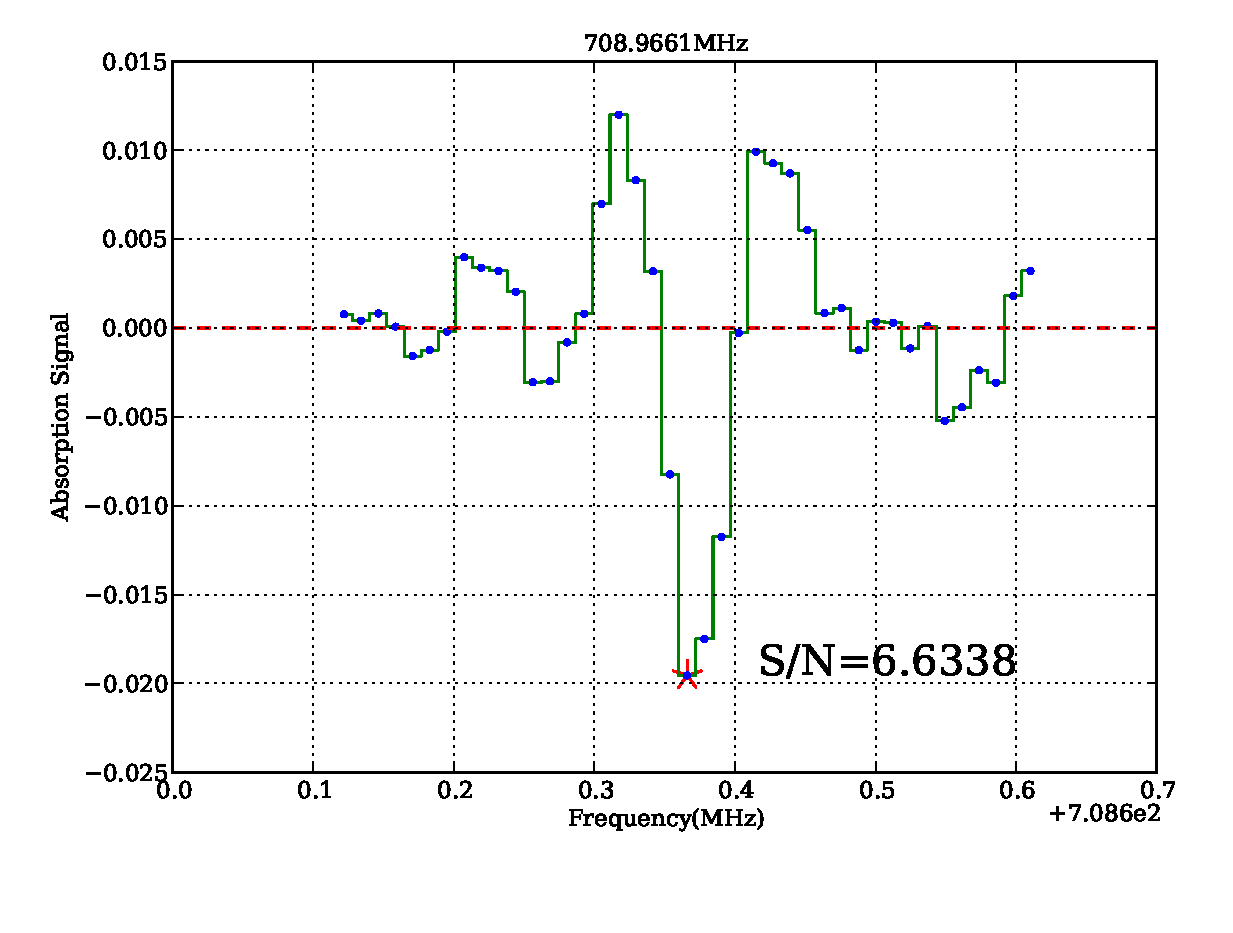
\includegraphics[width=8cm]{708966064_20_7_svd.eps}
%      %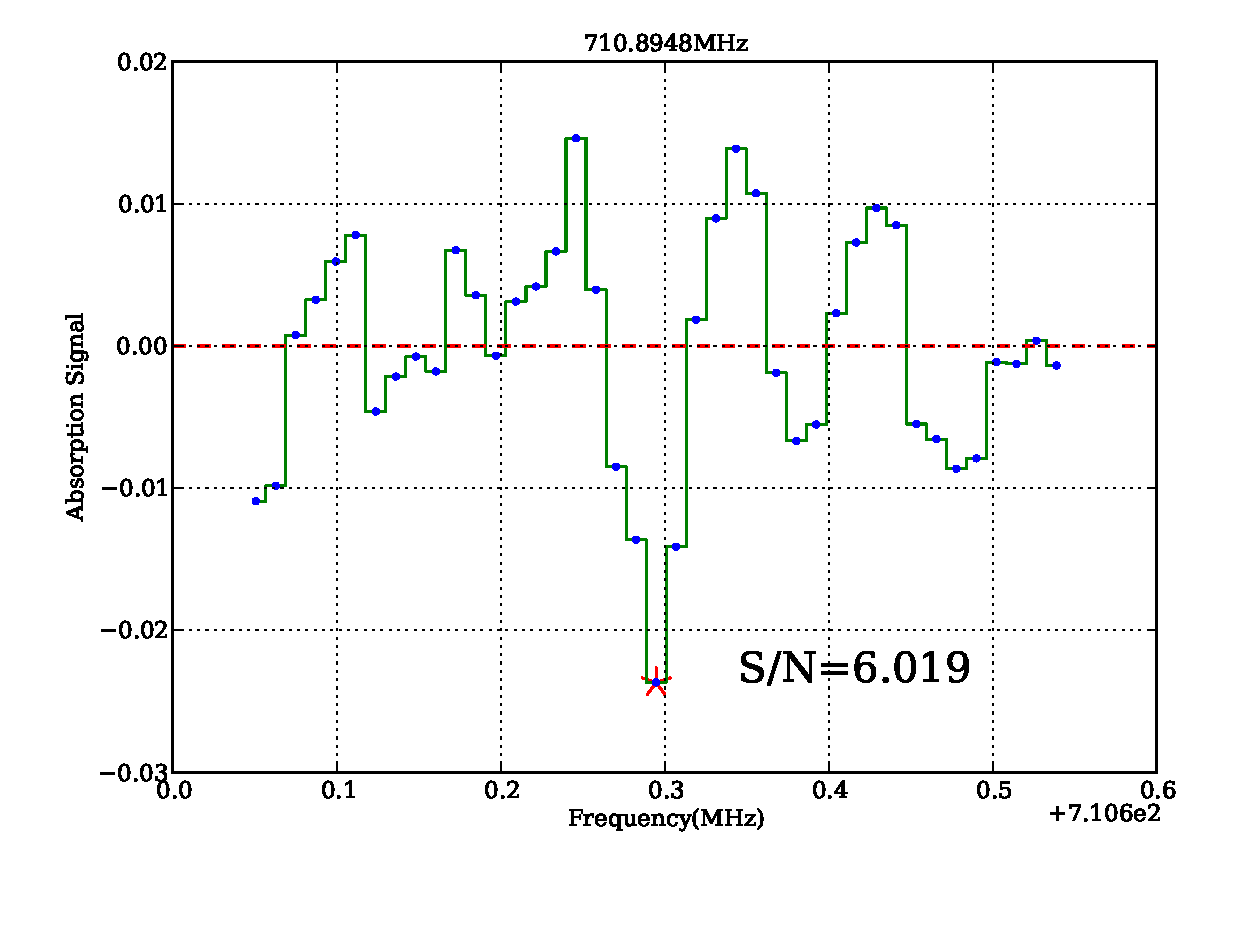
\includegraphics[width=8cm]{710894775_24_8_svd.eps}
%      %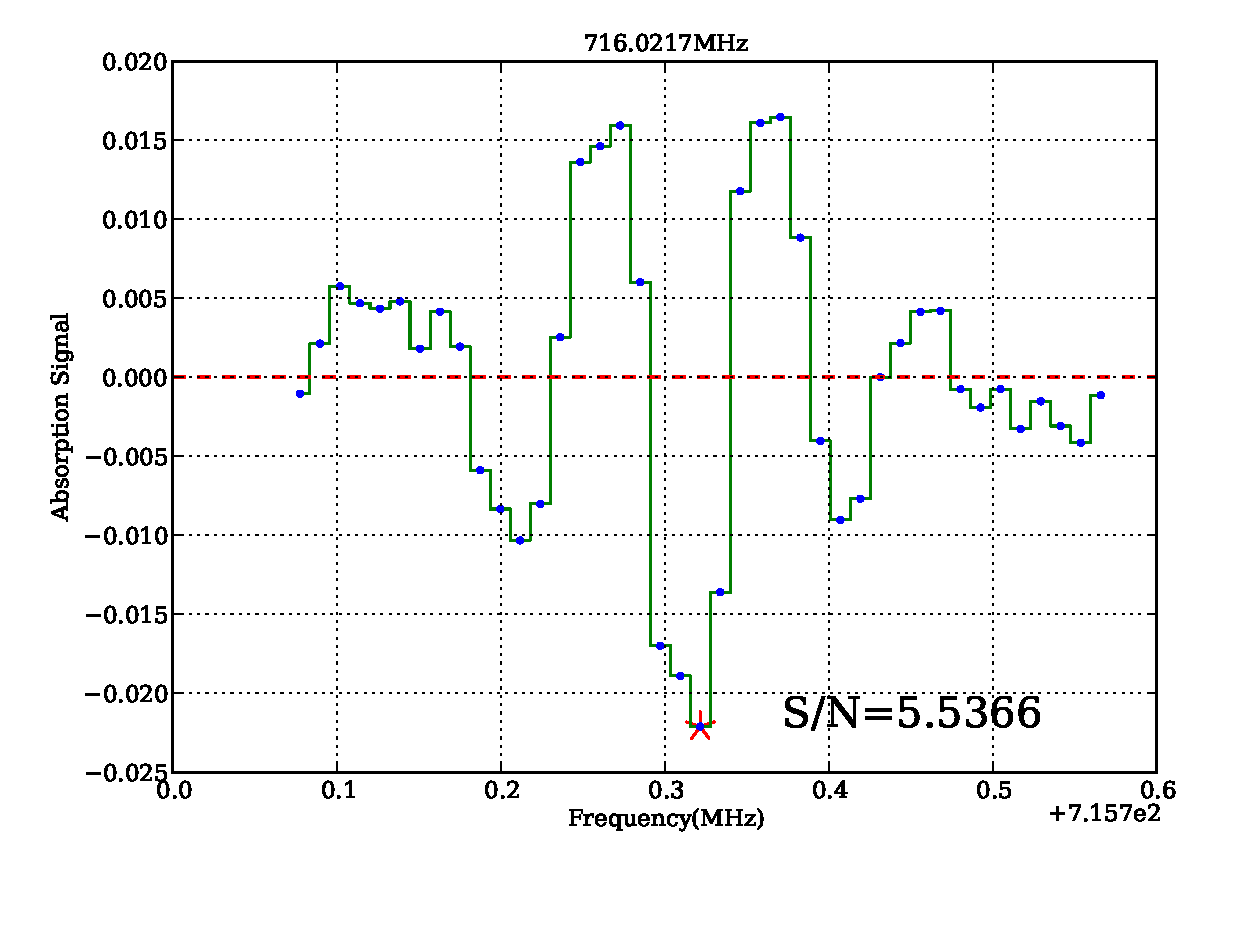
\includegraphics[width=8cm]{716021728_3_6_svd.eps}
%      %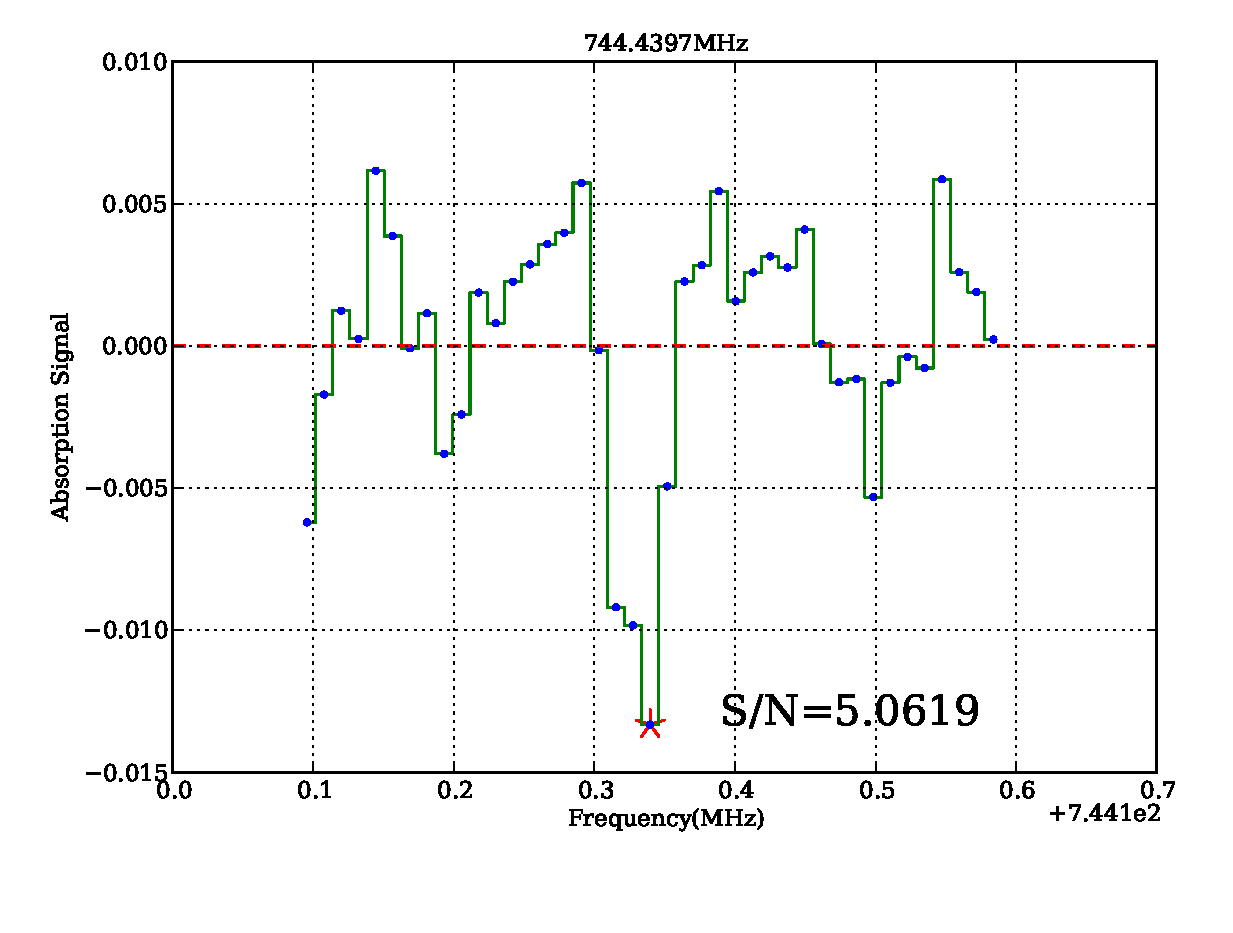
\includegraphics[width=8cm]{744439697_24_10_svd.eps}
%      %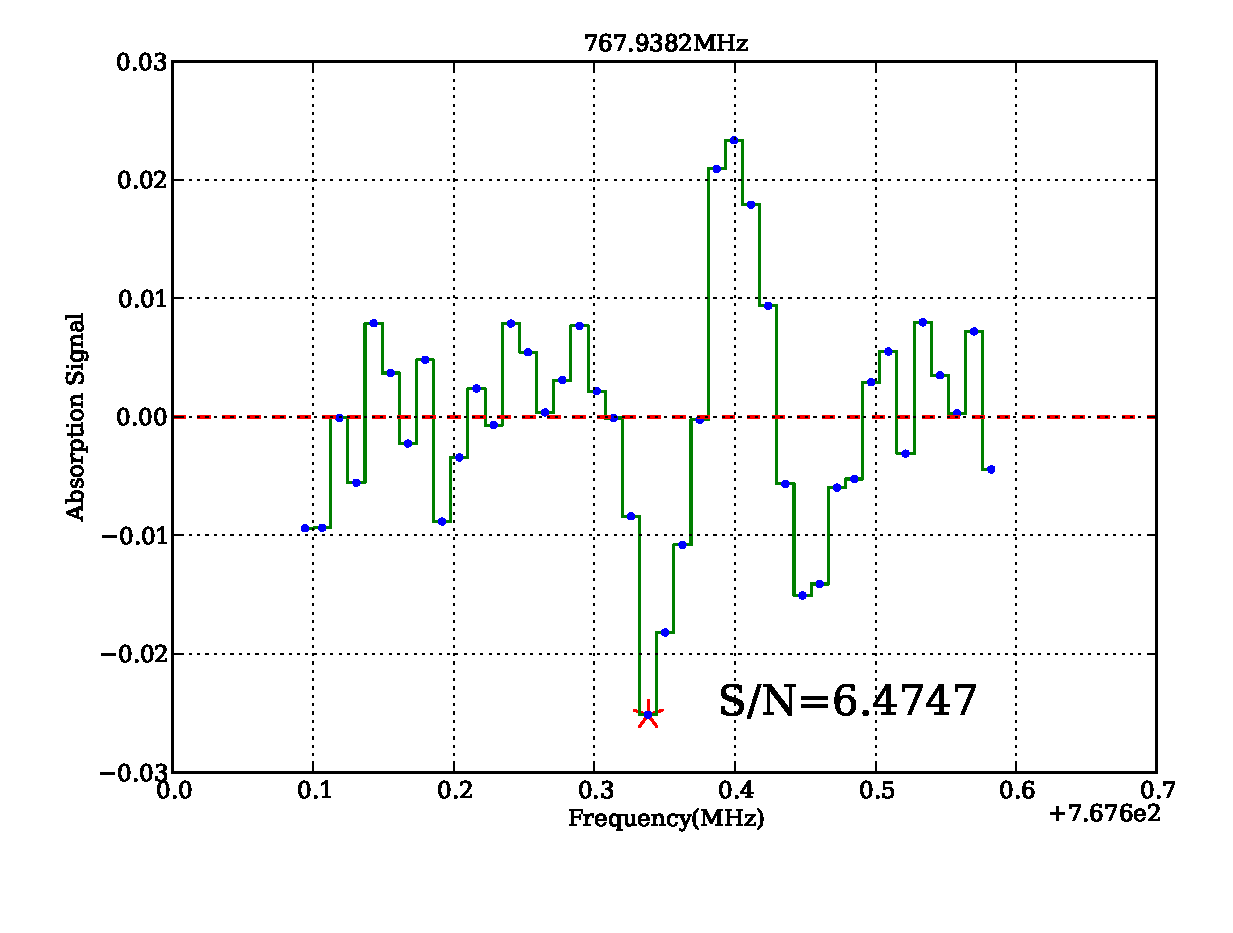
\includegraphics[width=8cm]{767938232_0_1_svd.eps}
%      %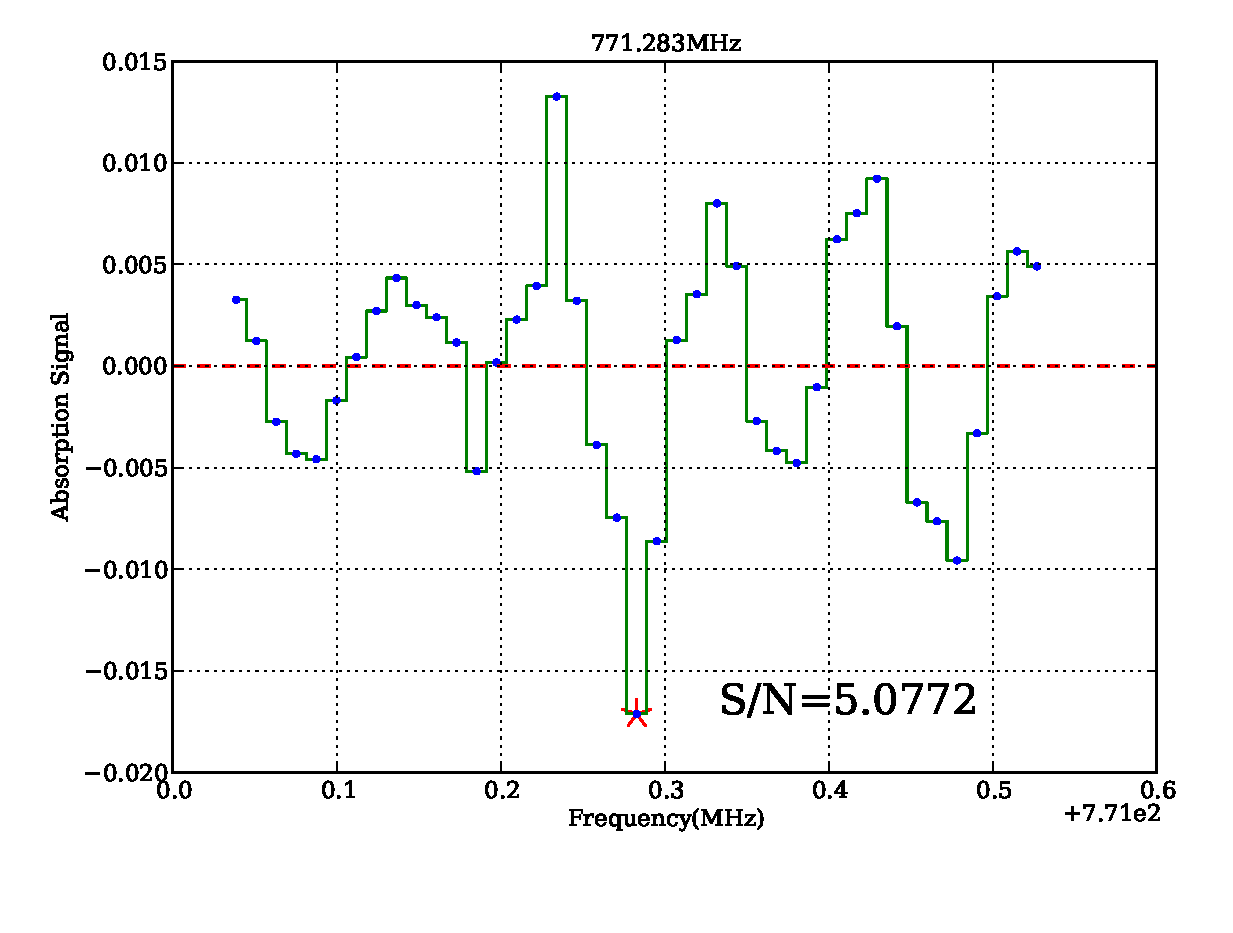
\includegraphics[width=8cm]{771282958_18_0_svd.eps}
%      %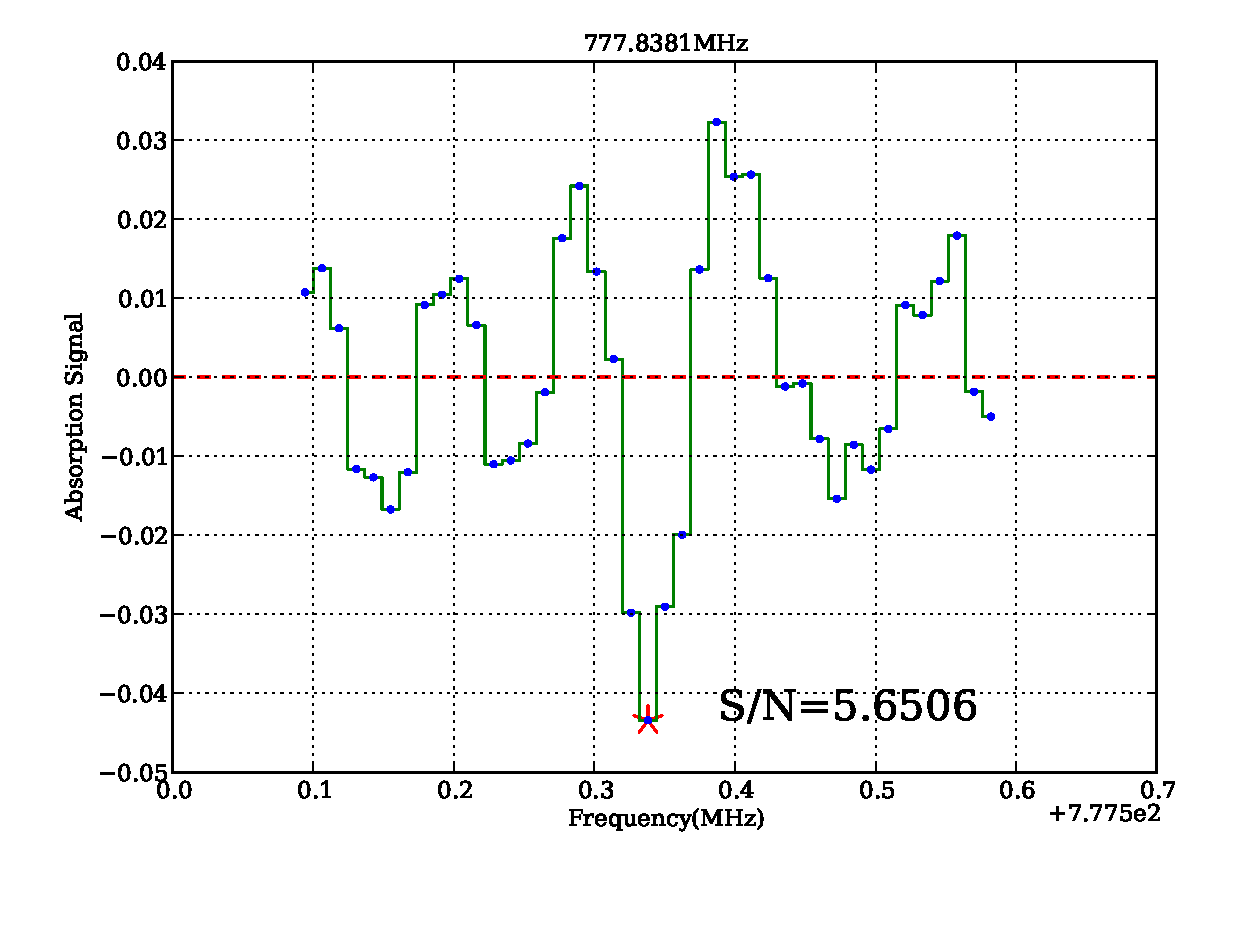
\includegraphics[width=8cm]{777838134_7_11_svd.eps}
%
%      %\caption{The local spectra of two 21 cm absorber candidates after subtracting the continuum.}
%      %\label{Fig.candidates}
%\end{figure}



\section{Proposed observations and Science}
We request a total of 12 hours allocation at the 700 -- 900 MHz band to follow up the candidate 21 cm absorber found in the 1hr field by our blind searching 
technique. The total observing time should be divided into two sections, each with a 6 hours allocation, separated by four months, in order to do a 
consistency check for the Doppler shift due to the Earth rotation. 
This follow-up observation will allow us to demonstrate the feasibility of our 
blind searching technique for 21 cm absorbers. If confirmed, this candidate 
would be the first HI absorber detected through 21 cm blind survey, without 
relying on an existing DLA catalog. 

Observations of 21 cm absorption lines will also provide information on the gas
properties of the absorber. We expect to constrain the combined quantity 
$N_{\rm HI}*c_f/T_{\rm spin}$, and to see if there is a systematic bias in the 
cool gas amount in the DLA-selected absorbers.



\section{Technical justification}

We are going to track the target position with GBT FP1 800 MHz receiver, which 
can cover frequency range from 680MHz to 920MHz. In order to achieve a higher
frequency resolution, two of the spectrometers of VEGAS backend are required.
One spectrometer works on mode 6, which have 187.5MHz bandwidth and 1.4kHz 
frequency resolution; the other spectrometer works on mode 19, which can 
achieve the highest frequency resolution at the frequency of the candidate. 

According to the absorption line we find in our blind searching, the signal to 
noise ratio is very high. The 1hr field has over 100 hours observation time, and is separated into 9 sub regions. Totally there are $30\times12$ pixels in each region. The integration time for
each pixel is about 17 minutes in average. According to the GBT 
sensitivity calculator, about 90 minutes effective integration time is needed 
to achieve over $10\sigma$ sensitivity. Considering frequency or position 
switching, reference observation, calibration, as well as the effect of RFI, 
about 6 hours observation time is needed.

In order to minimize RFI, we prefer to observe at night, with higher elevation, but it is not required. Only one of the two sessions can be night time.
Also with our well developed off-line data analysis code, we can flag out 
the remaining RFI, which is already been used in our previous analysis.

\section{Student training}
There are currently a number of graduate students working on the blind searching 
for 21 cm absorbers at GBT.  One of them, Wenkai HU, is the PI of this proposal and is developing 
the blind searching technique for his first science project, and going to 
keep working on 21 cm absorber related research. 

\section{Conclusion}
We have proposed to use the 700 -- 900 MHz band to follow up 
one 21 cm absorber candidate found by our blind searching technique. 
We aim to confirm the existence of these two absorbers, and to demonstrate 
the feasibility of the blind searching technique. This technique will 
be useful for seaching for more 21 cm absorbers in future
21 cm surveys, without relying on the existing DLA catalogs, 
thus avoiding the selection bias. This measurement
will also put constraints on the gas properties of the absorbers.

\bibliography{GBT_absorber_proposal}
\bibliographystyle{apsrev}
%\clearpage

\section{Appendix}

\begin{figure*}[h]
(1)\subfigure{%\label{Fig.sub.1}
%part5
      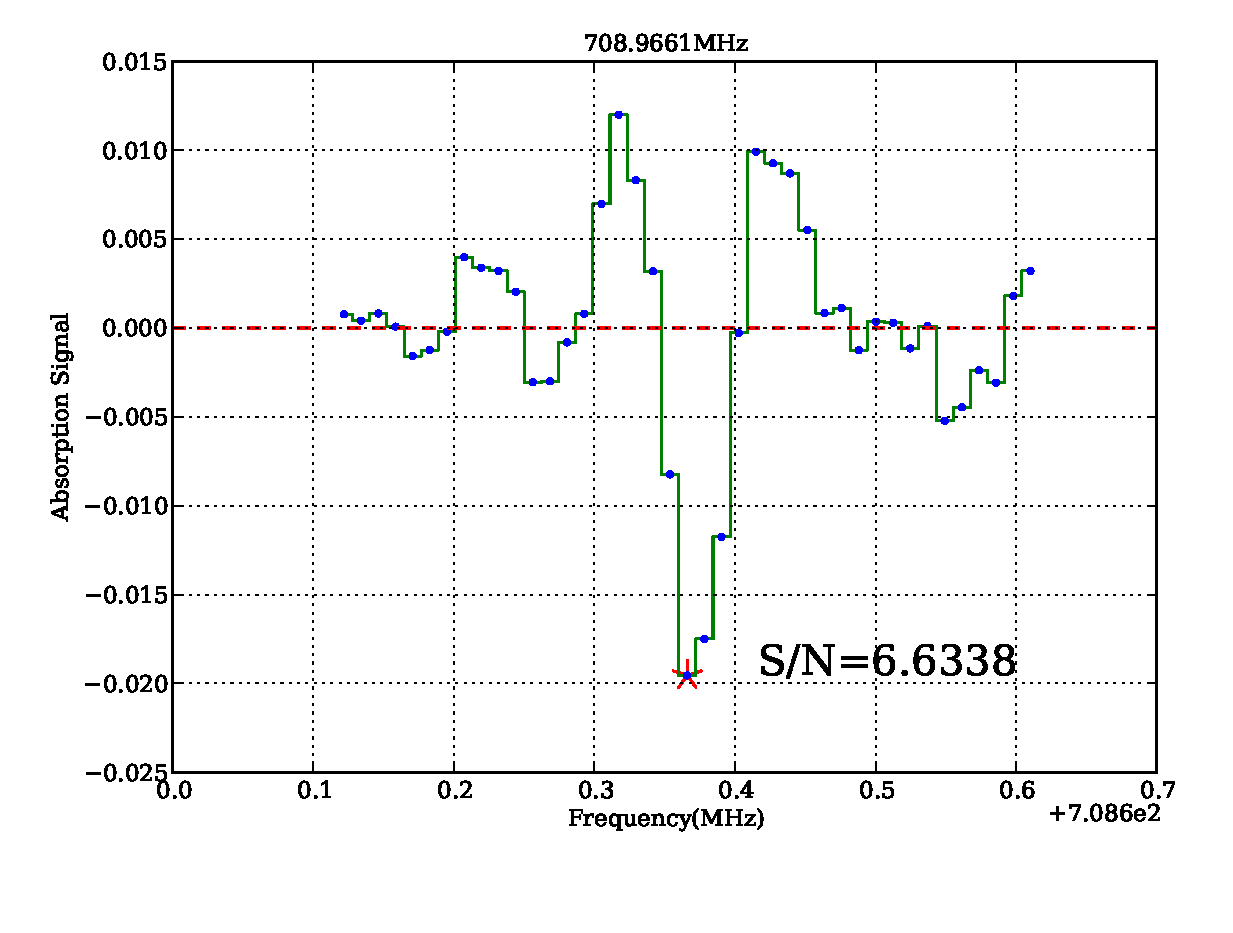
\includegraphics[width=6cm]{708966064_20_7_svd.eps}}
      \hspace{1.1ex}
      \vspace{-1.2ex}
(2)\subfigure{%\label{Fig.sub.1}
%part1
      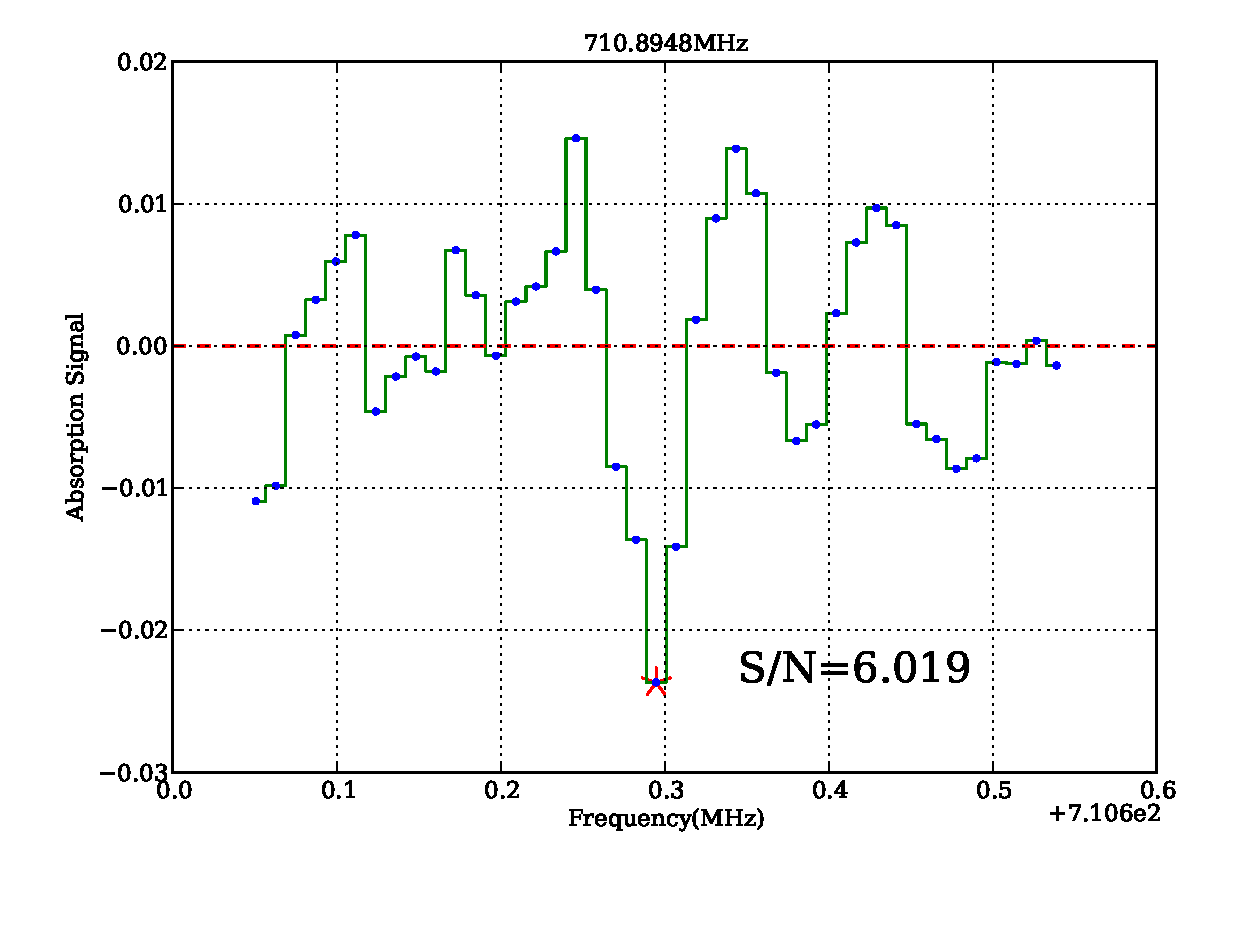
\includegraphics[width=6cm]{710894775_24_8_svd.eps}}
      \hspace{1.1ex}
      \vspace{-1.2ex}

(3)\subfigure{%\label{Fig.sub.1}
%part3
      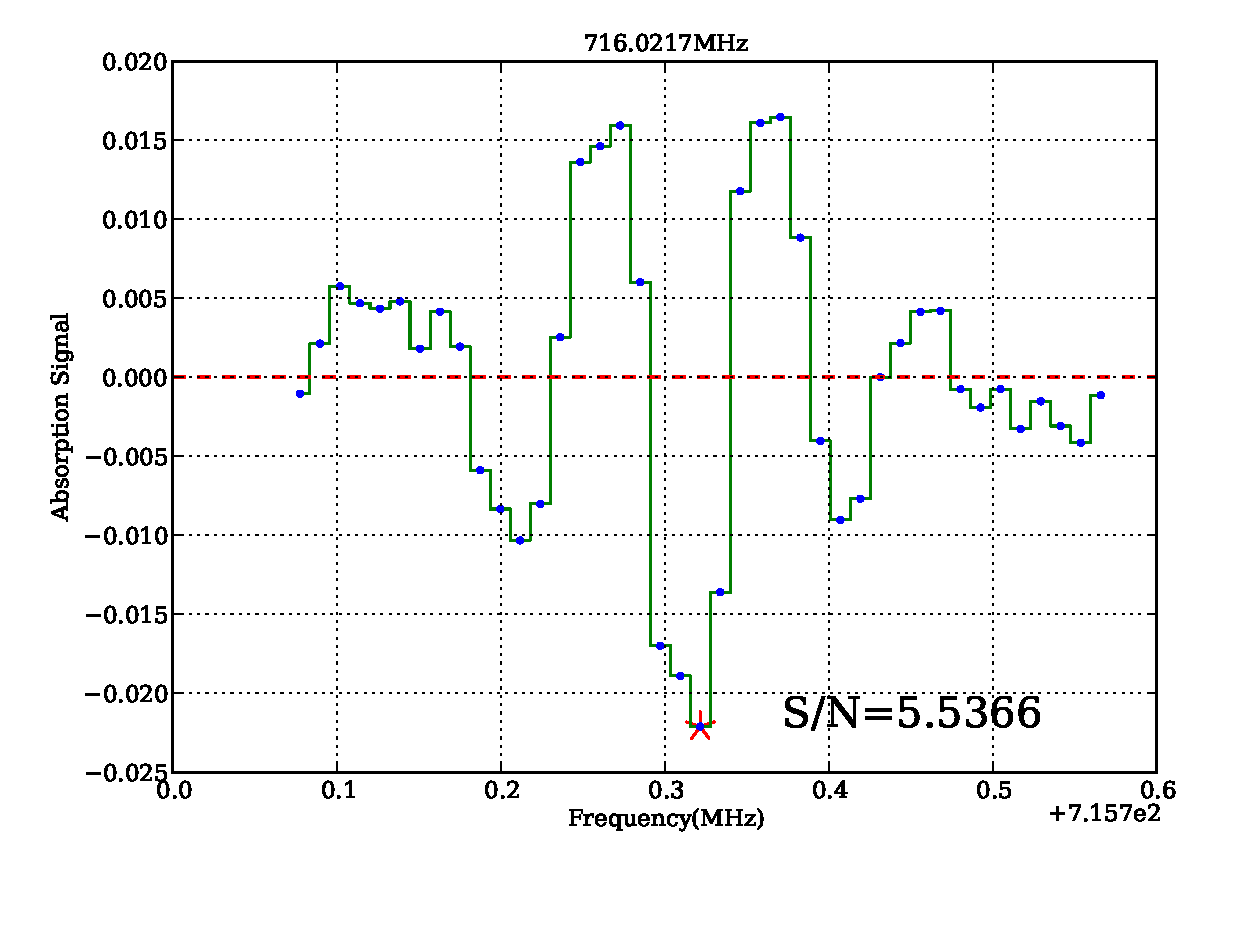
\includegraphics[width=6cm]{716021728_3_6_svd.eps}}
      \hspace{1.1ex}
      \vspace{-1.2ex}
(4)\subfigure{%\label{Fig.sub.1}
%part5
      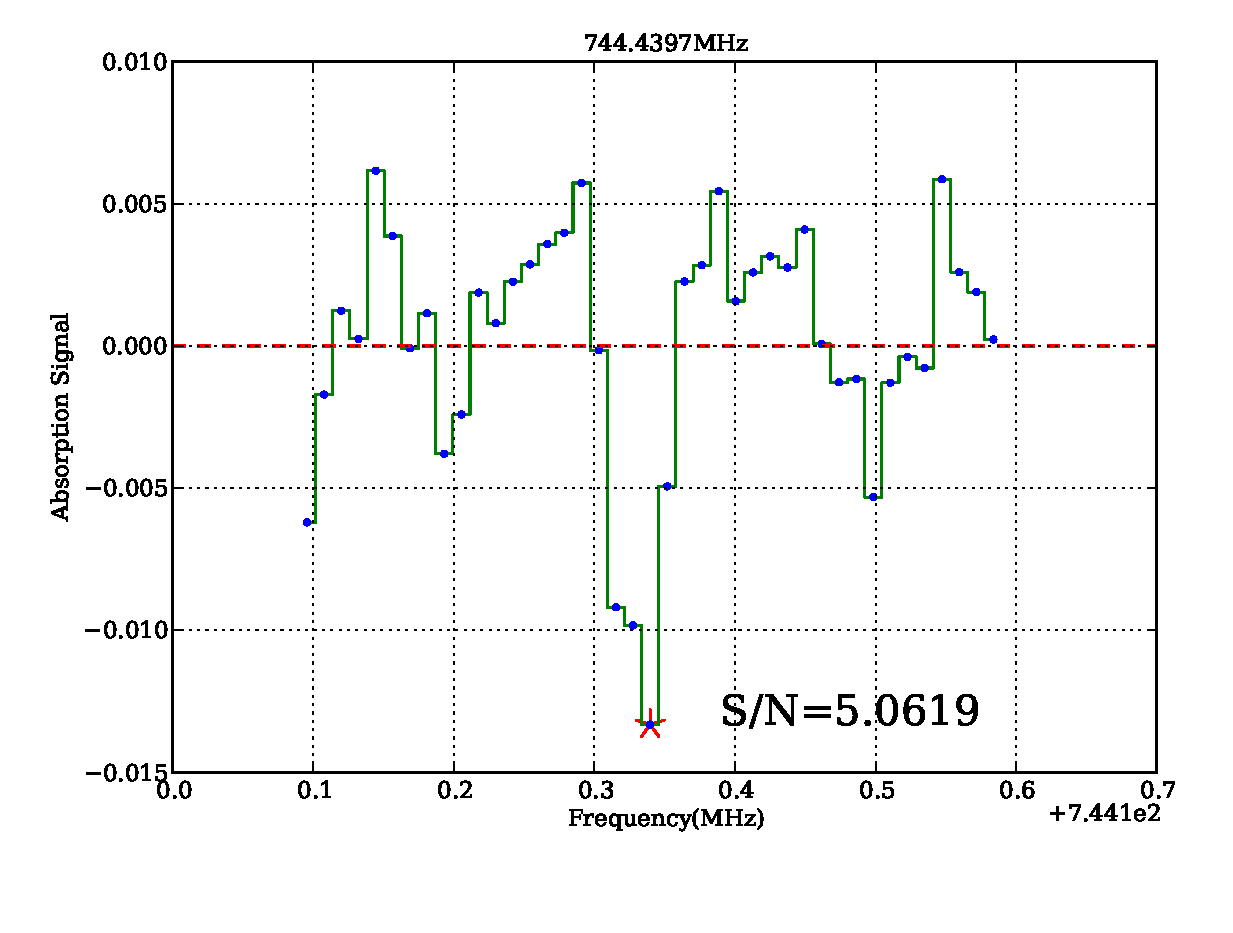
\includegraphics[width=6cm]{744439697_24_10_svd.eps}}
      \hspace{1.1ex}
      \vspace{-1.2ex}
(5)\subfigure{%\label{Fig.sub.1}
%part5
      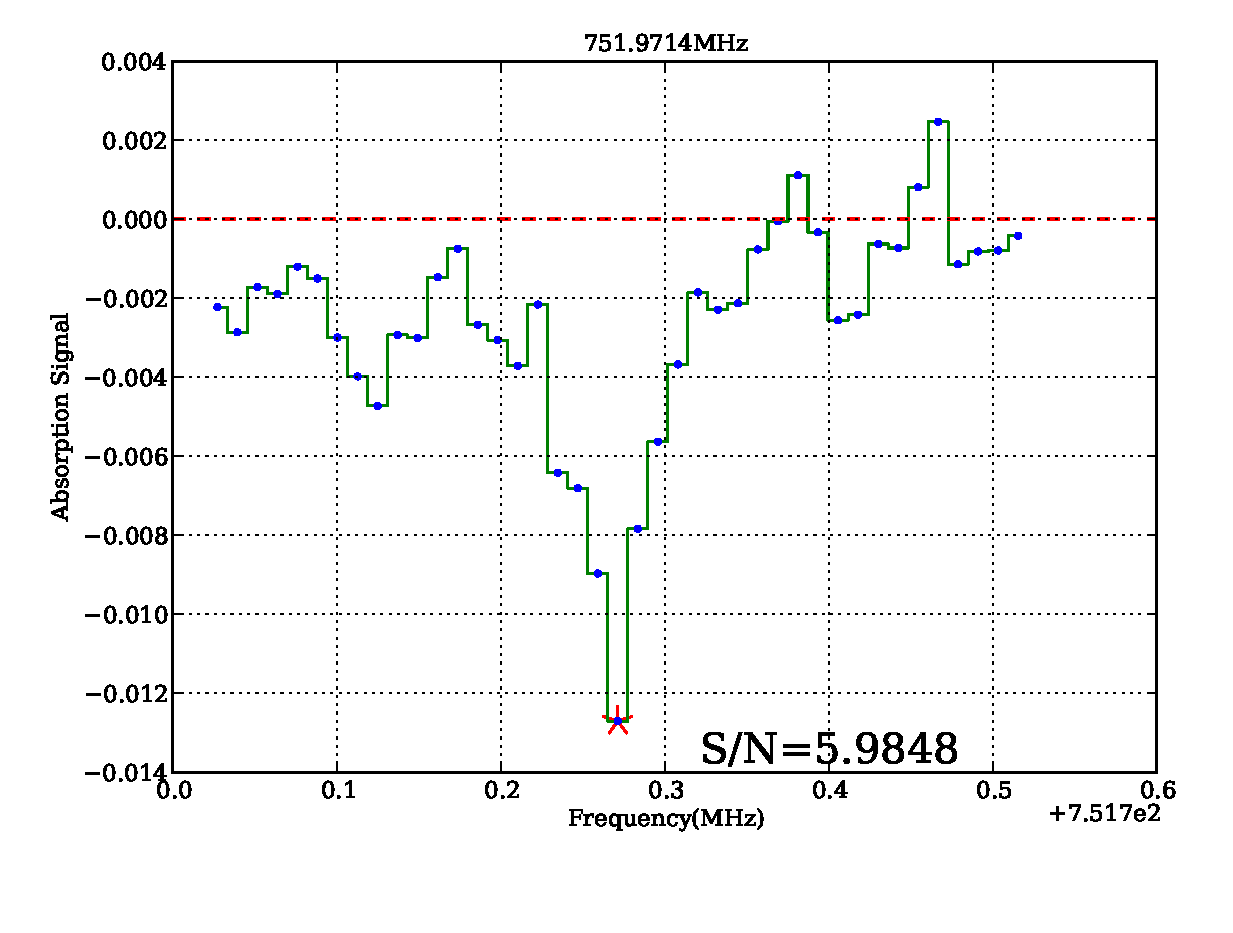
\includegraphics[width=6cm]{751971435_22_7_svd.eps}}
      \hspace{1.1ex}
      \vspace{-1.2ex}
(6)\subfigure{%\label{Fig.sub.1}
%part3
      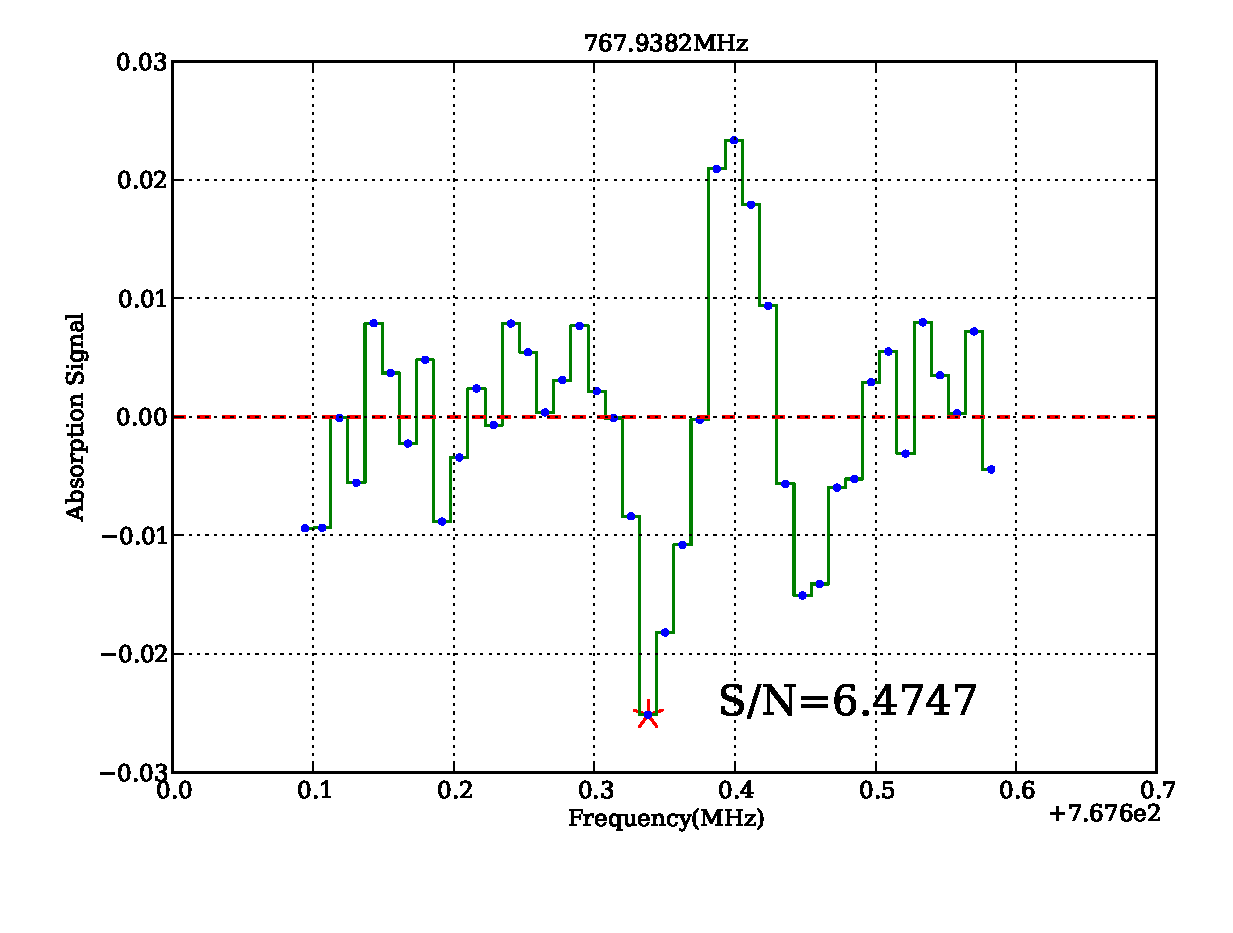
\includegraphics[width=6cm]{767938232_0_1_svd.eps}}
      \hspace{1.1ex}
      \vspace{-1.2ex}
(7)\subfigure{%\label{Fig.sub.1}
%part2
      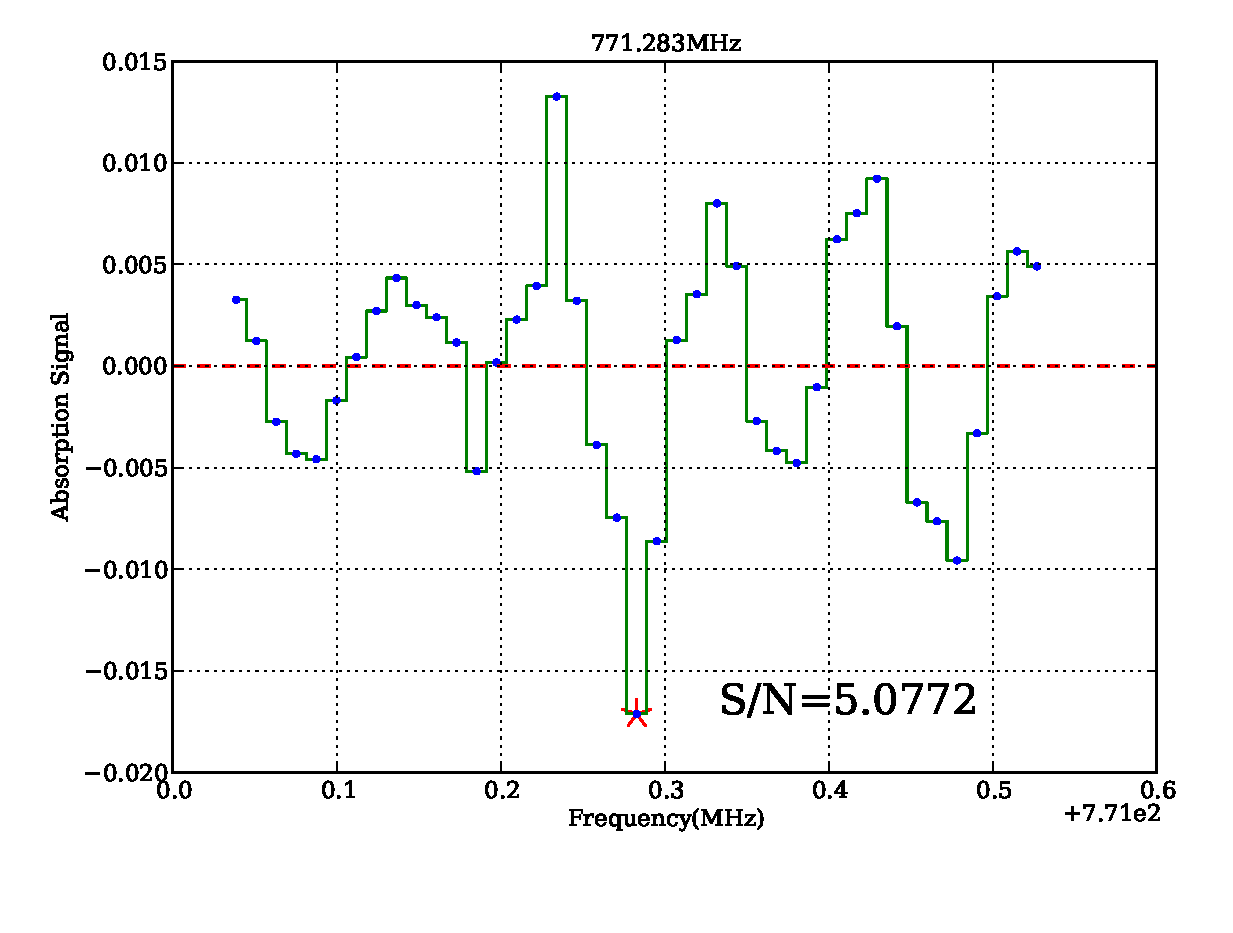
\includegraphics[width=6cm]{771282958_18_0_svd.eps}}
      \hspace{1.1ex}
      \vspace{-1.2ex}
(8)\subfigure{%\label{Fig.sub.1}
%part9
      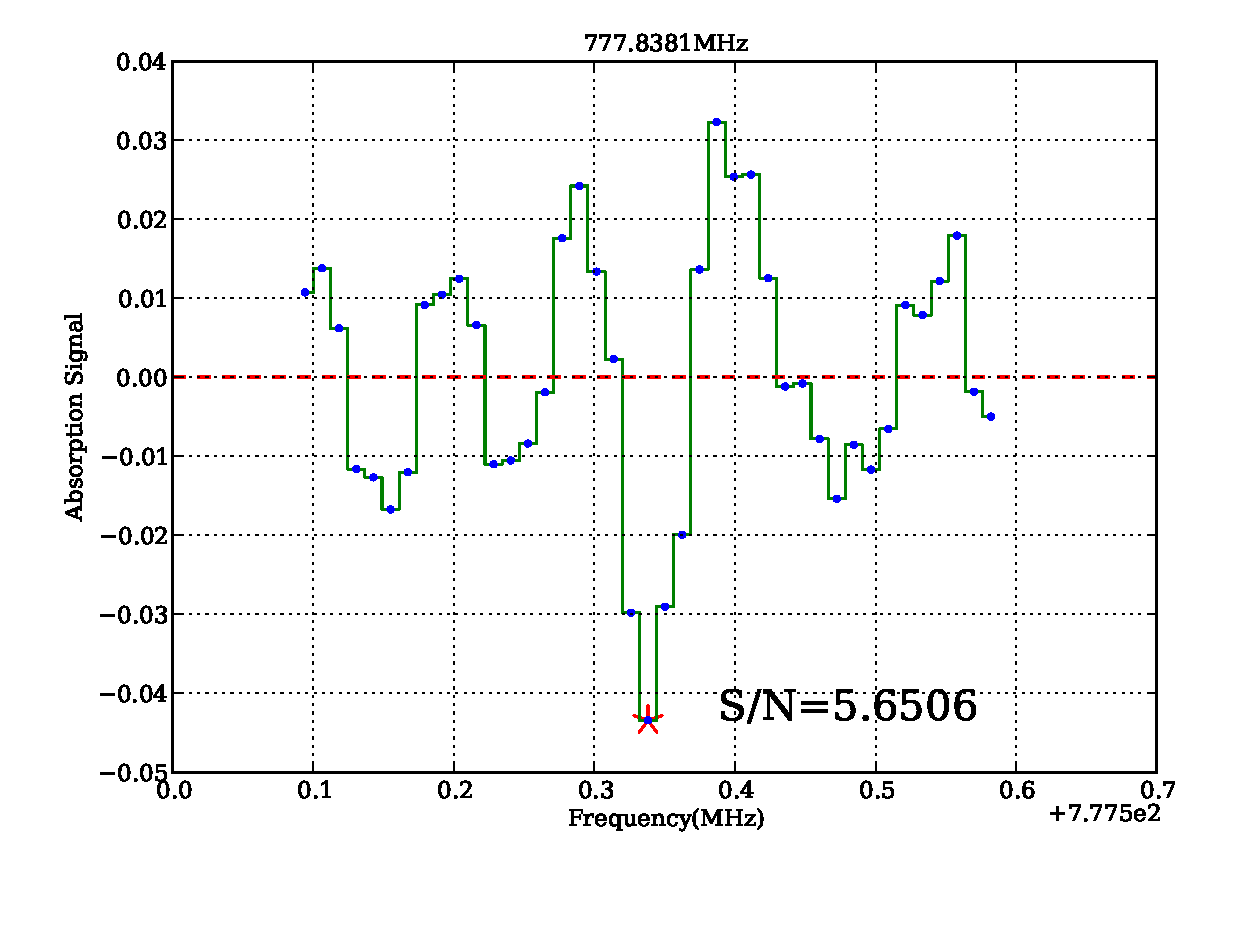
\includegraphics[width=6cm]{777838134_7_11_svd.eps}}
      %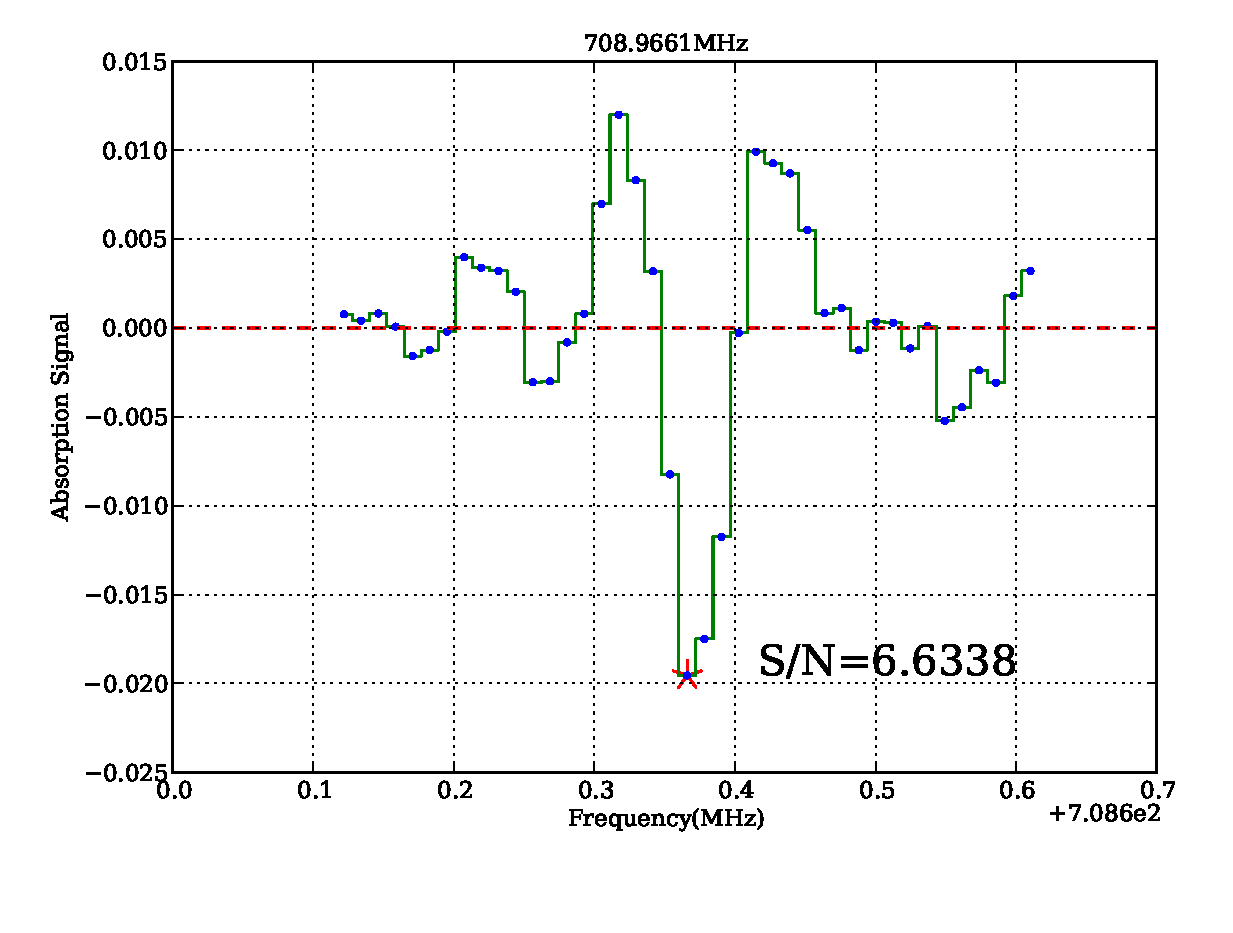
\includegraphics[width=8cm]{708966064_20_7_svd.eps}
      %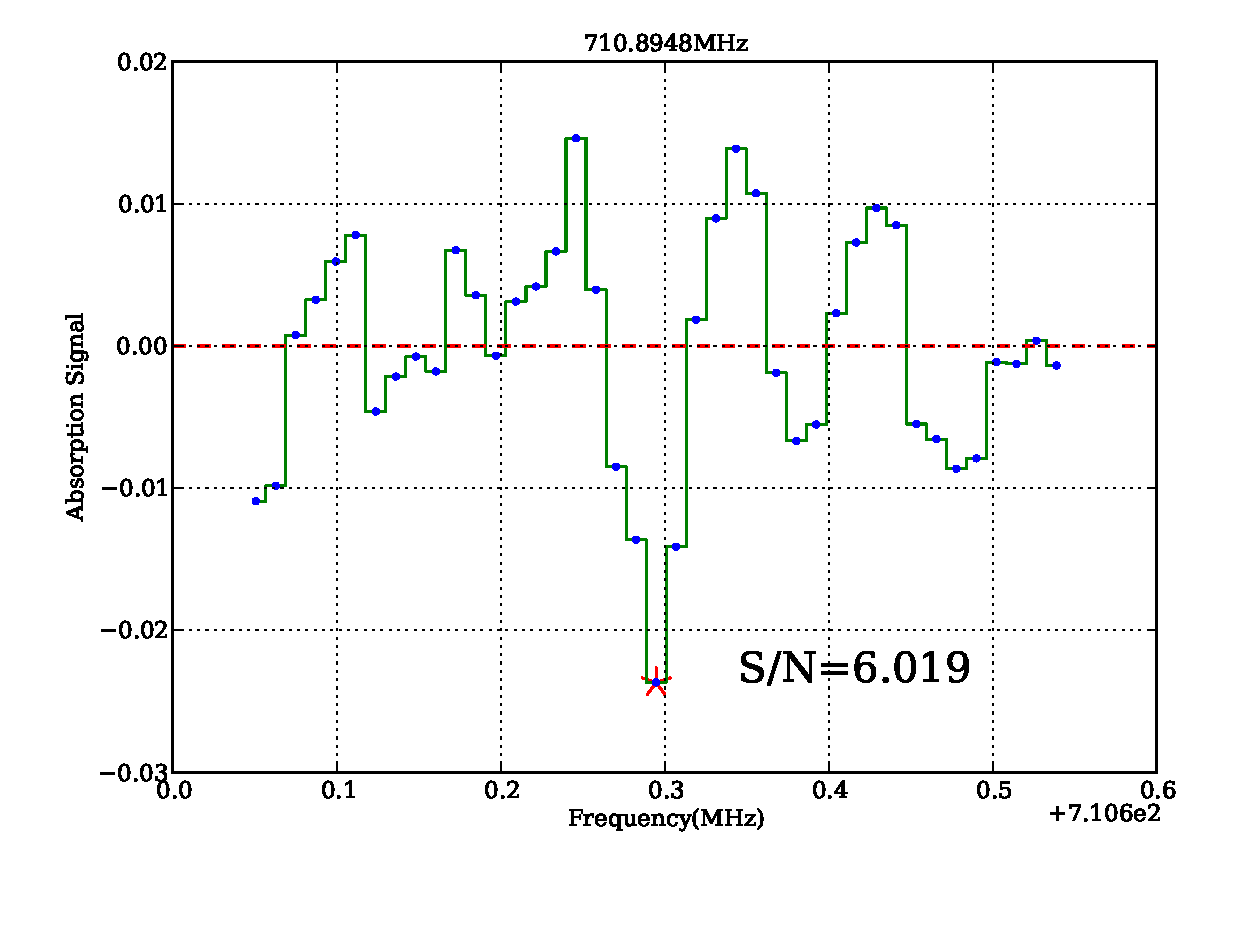
\includegraphics[width=8cm]{710894775_24_8_svd.eps}
      %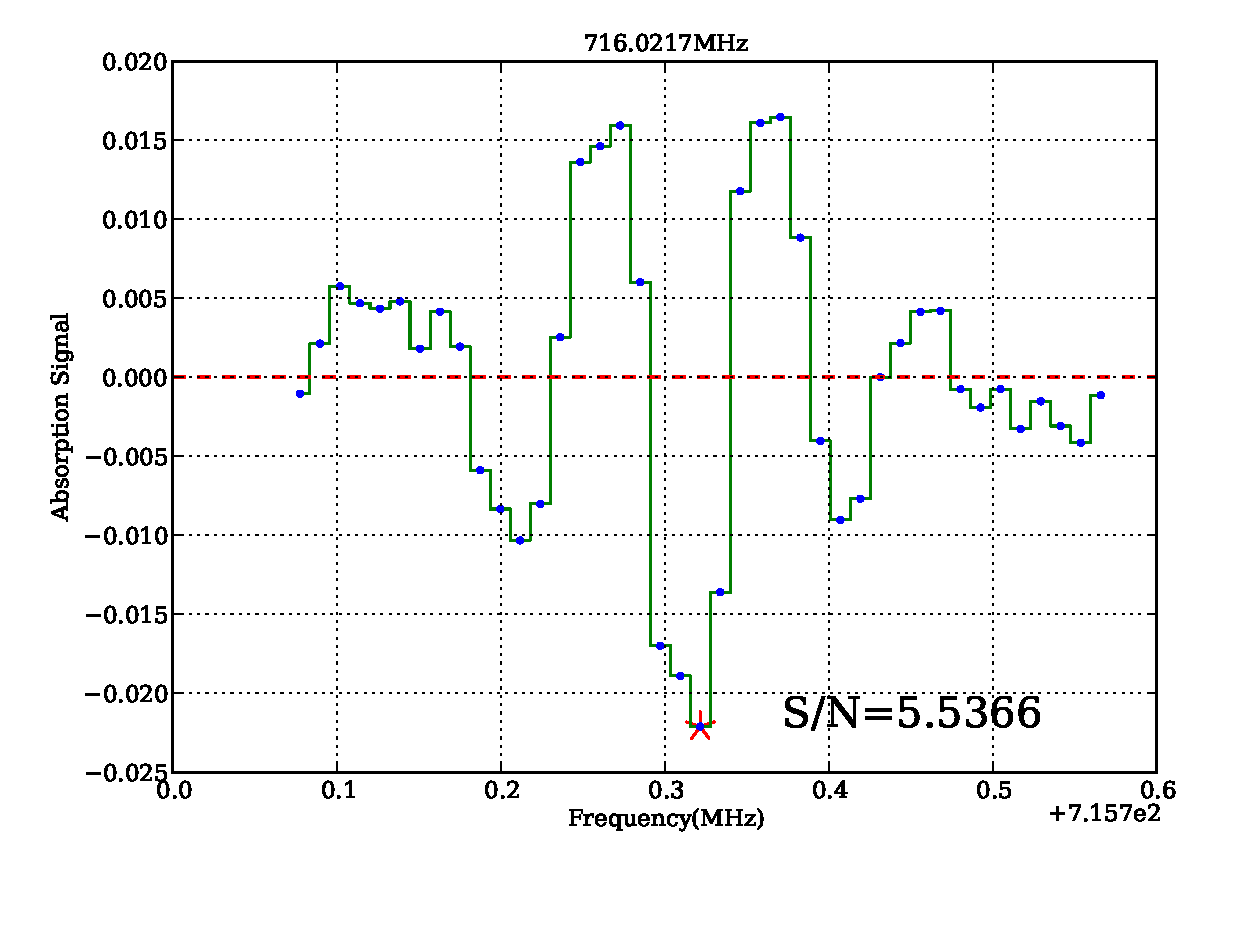
\includegraphics[width=8cm]{716021728_3_6_svd.eps}
      %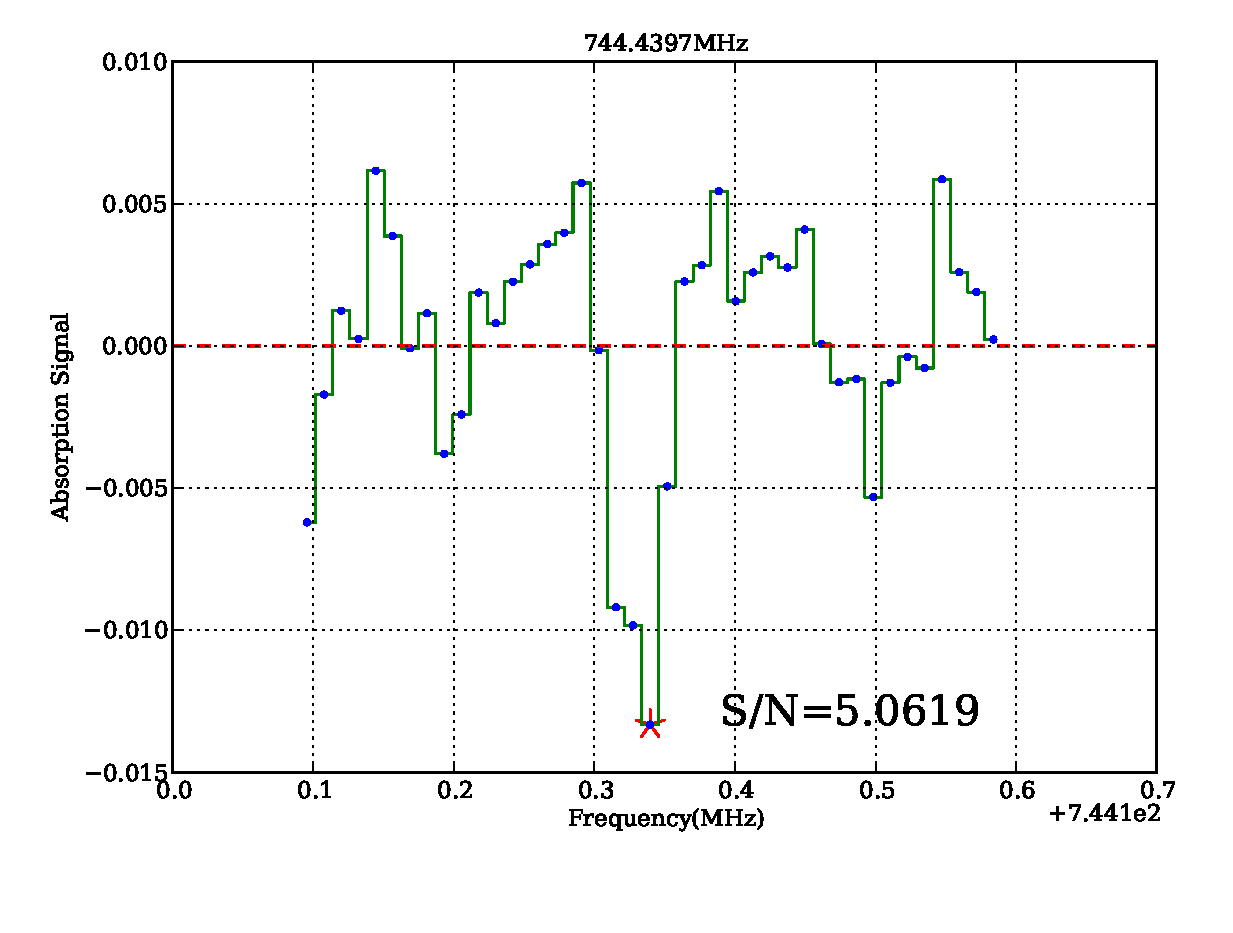
\includegraphics[width=8cm]{744439697_24_10_svd.eps}
      %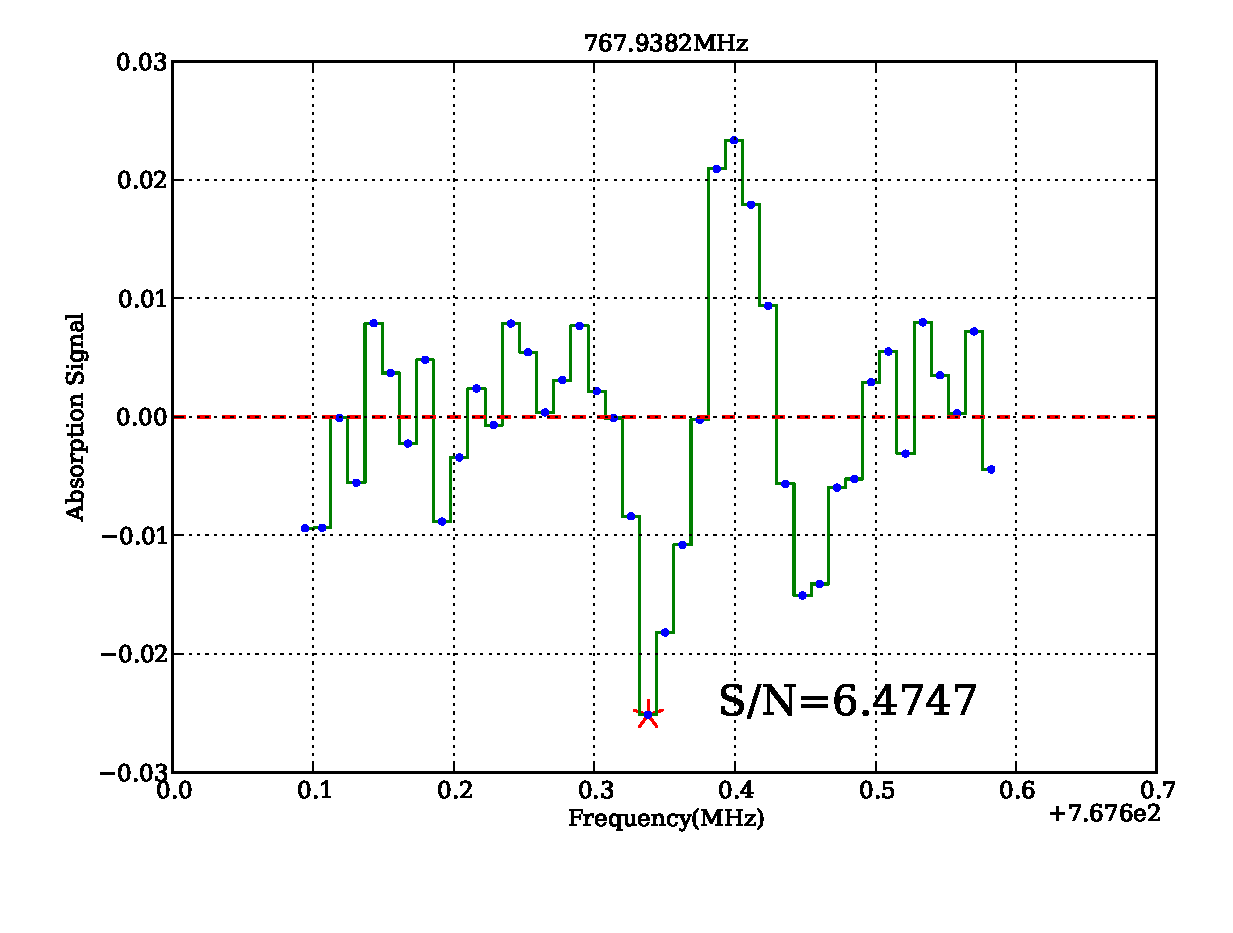
\includegraphics[width=8cm]{767938232_0_1_svd.eps}
      %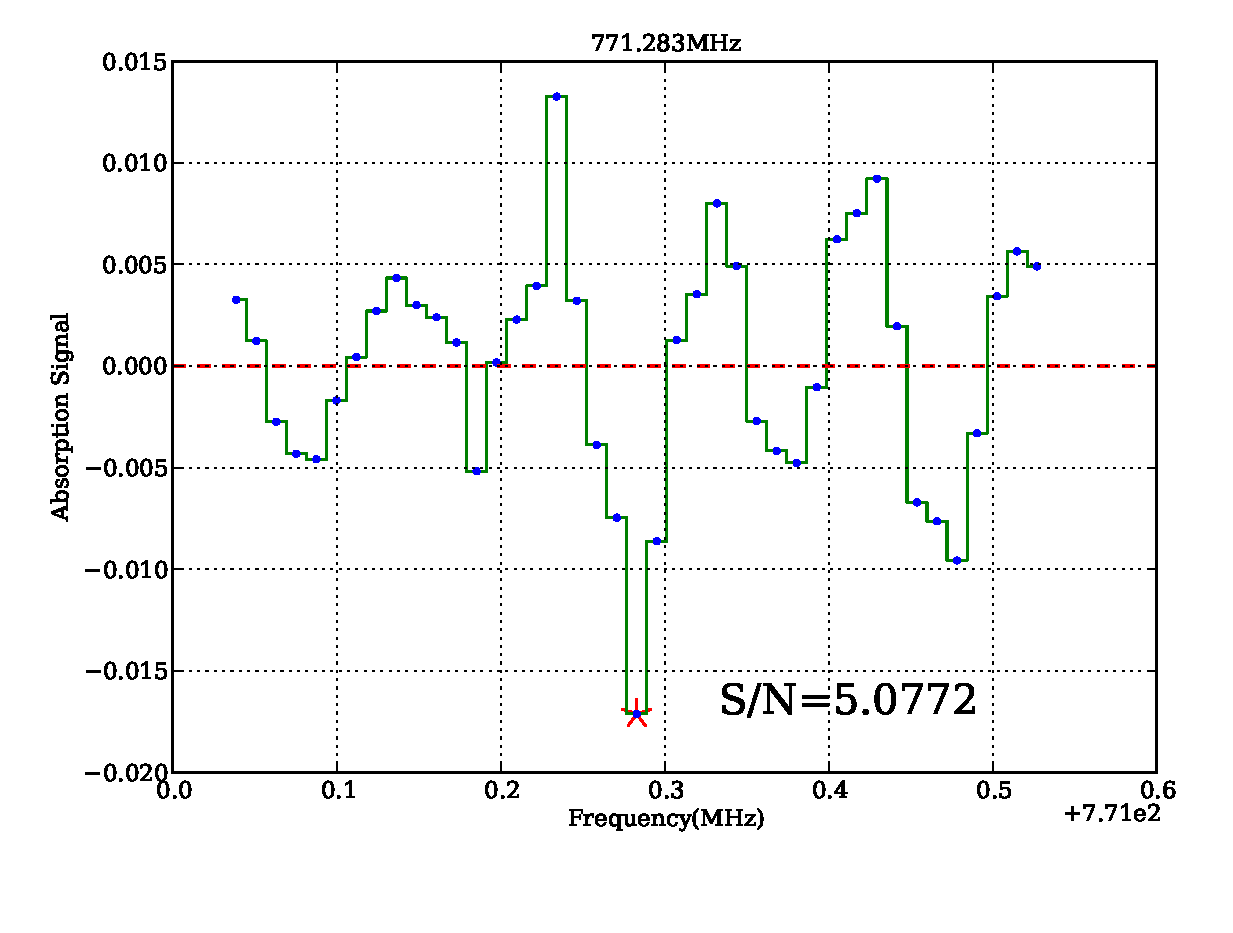
\includegraphics[width=8cm]{771282958_18_0_svd.eps}
      %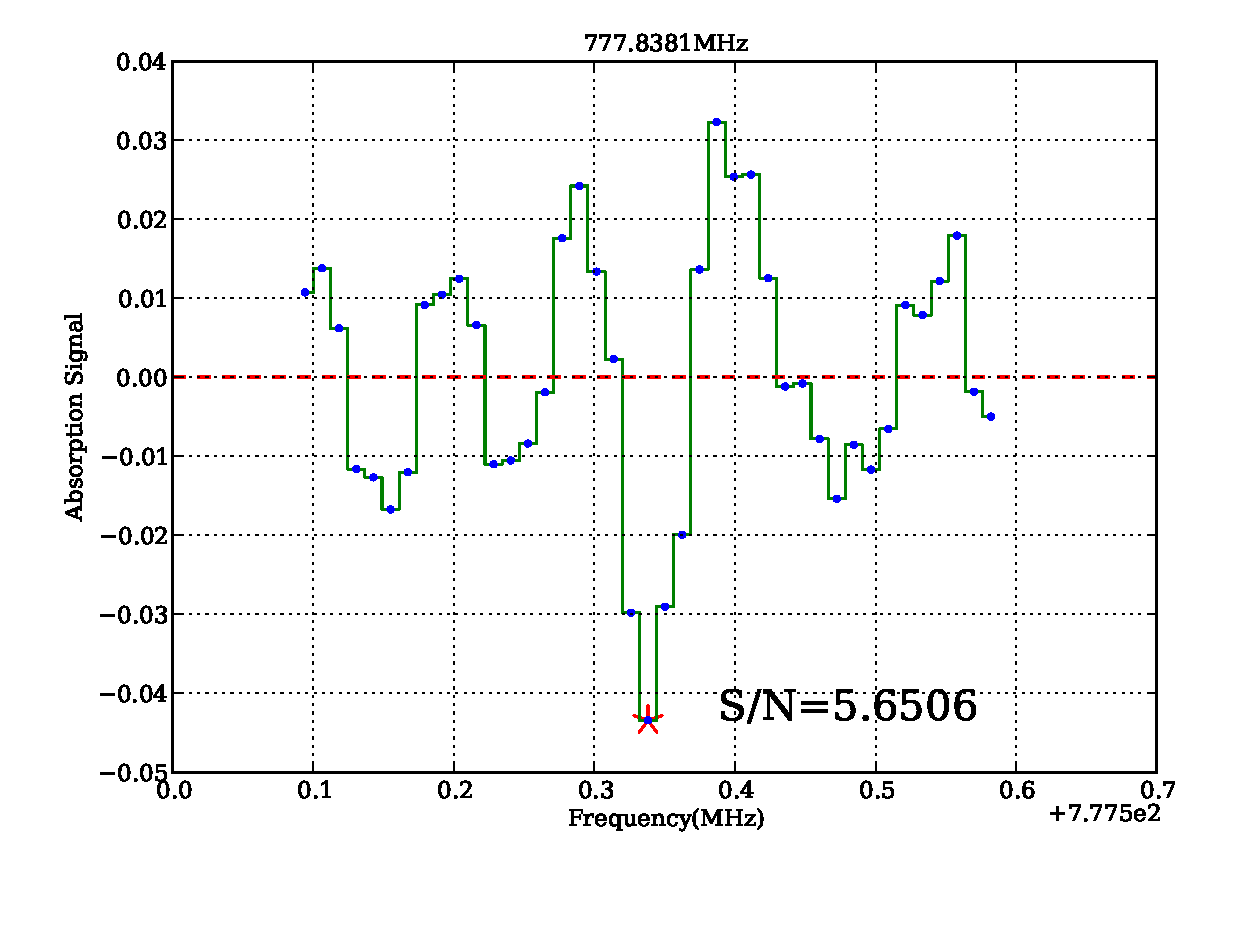
\includegraphics[width=8cm]{777838134_7_11_svd.eps}

      \caption{The local spectra of two 21 cm absorber candidates after subtracting the continuum.(1).RA = 0h54m00s, DEC = $1^{\circ}10^\prime$, 708.9661MHz, (2).RA = 0h36m41s, DEC = $3^{\circ}20^\prime$, 710.8948MHz, (3).RA = 1h02m39s, DEC = $3^{\circ}00^\prime$, 716.0217MHz (4).RA = 0h56m40s, DEC = $1^{\circ}40^\prime$, 744.4397MHz, (5).RA = 0h55m20s, DEC = $1^{\circ}10^\prime$, 751.9714MHz, (6).RA = 1h00m39s, DEC = $2^{\circ}10^\prime$, 767.9382MHz, (7).RA = 00h52m40s, DEC = $2^{\circ}00^\prime$, 771.2830MHz (8).RA = 1h05m20s, DEC = -$00^{\circ}10^\prime$, 777.8381MHz}
      \label{Fig.candidates}
\end{figure*}
\end{document}



